% biber
\documentclass[paper=letter, fontsize=12pt]{article}

\usepackage[english]{babel} % English language/hyphenation
\usepackage{amsmath,amsfonts,amsthm} % Math packages
%\usepackage[section]{placeins}  % prevent figures / eqns / tables
                                % from slipping out of section.
\usepackage{sectsty} % Allows customizing section commands
\allsectionsfont{\normalfont\scshape} % Make all sections centered,
                                                 % the default font and small
                                                 % caps

\usepackage{fancyhdr} % Custom headers and footers

% algorithms
\usepackage{algorithm}
\usepackage[compatible]{algpseudocode}

\usepackage{ragged2e} % Text alignment
\usepackage[margin=1in]{geometry} % 1 inch margins
\usepackage{tikz} % Not always necessary, but allows very customizable
                  % figures / object placement
\usepackage{enumitem} % get more out of enumerate

% begin additional packages
\usepackage{booktabs}
\usepackage{csquotes}
\usepackage{hyperref}
\usepackage{blindtext}
\usepackage{subfig}
\usepackage[
    backend=biber,
    url=false,
    doi=true,
    eprint=true
]{biblatex}
\addbibresource{./references.bib}
%   Appendix at end of Article
\usepackage{environ}
\newtoks\mainnotetoks
\newtoks\tempnotetoks
\newtoks\prenotetoks
\newtoks\postnotetoks

\NewEnviron{appendixatend}{%
  \tempnotetoks=\expandafter{\BODY}%
  \edef\notetemp{%
    \the\mainnotetoks % what was already stored
    \the\prenotetoks % text before the new note
    \the\tempnotetoks % the current note
    \the\postnotetoks % text after the new note
  }%
  % update \mainnotetoks
  \global\mainnotetoks=\expandafter{\notetemp}%
}
\newcommand\includeappendices{%
  \appendix
  \renewcommand{\thesection}{\Alph{section}}
  \section{Appendix}
  \the\mainnotetoks}

% set the pre and post note
\prenotetoks={}
\postnotetoks={}
%   End Appendix at end of Article

% end additional packages

% Header and Footers
\pagestyle{fancyplain} % Makes all pages in the document conform to the custom
                       % headers and footers
\fancyhead{} % No page header
\fancyfoot[L]{} % Empty left footer
\fancyfoot[C]{} % Empty center footer
\fancyfoot[R]{\thepage} % Page numbering for right footer
\renewcommand{\headrulewidth}{0pt} % Remove header underlines
\renewcommand{\footrulewidth}{0pt} % Remove footer underlines
\setlength{\headheight}{13.6pt} % Customize the height of the header

% Number all figs, eqns, and tables within the section
\numberwithin{equation}{section} % Number equations within sections
\numberwithin{figure}{section} % Number figures within sections
\numberwithin{table}{section} % Number tables within sections

\setlength\parindent{4pt} % 4pt indentation for paragraphs
\setlength{\parskip}{\baselineskip} % adds some spacing in between paragraphs

\newcommand{\horrule}[1]{\rule{\linewidth}{#1}} % Create horizontal rule command
                                                % with 1 argument of height
\newcommand{\fancyline}{\\ \horrule{0.5pt} \vspace{0.1cm}} % fancy line to put
                                                           % under questions

%  Some commands for algorithm environments
\renewcommand{\algorithmicrequire}{\textbf{Input:}}
\renewcommand{\algorithmicensure}{\textbf{Output:}}
\renewcommand{\algorithmicforall}{\textbf{for each}}
\newcommand{\algorithmiccontinue}{\textbf{continue}}
\algloopdefx{RETURN}[1][]{\textbf{return} #1}

% useful math shortcuts
\newcommand{\lagr}[1]{\mathcal{L}\left( #1 \right)}
\newcommand{\expval}[1]{E\left[#1\right]}
\newcommand{\var}[1]{\text{var}\left(#1\right)}
\newcommand{\abs}[1]{\left|#1\right|}
\renewcommand{\det}[1]{\text{det}\left(#1\right)}
\newcommand{\diag}[1]{\text{diag}\left[#1\right]}

% begin additional definitions and commands
\DeclareMathOperator*{\argmax}{arg\,max}
\DeclareMathOperator*{\argmin}{arg\,min}
% end additional definitions and commands

%-------------------------------------------------------------------------------
%	TITLE SECTION
%-------------------------------------------------------------------------------

\title{
\normalfont \normalsize
\textsc{RICE UNIVERSITY COMP340} \\ [25pt]
\horrule{0.5pt} \\[0.4cm] % Thin top horizontal rule
\huge Auto Segmentation \\ % The assignment title
\horrule{2pt} \\[0.5cm] % Thick bottom horizontal rule
}

\author{Will LeVine \& Cole Morgan}

\date{\normalsize\today}

\begin{document}

\maketitle

\begin{abstract}
    We present a unique pipeline to segment individual automobiles in
    photographs, and to perform additional feature tagging.  The pipeline
    consists of aggressive downsampling to limit computing power requirements,
    followed by a binarization of pixels represented by several layers of linear
    and non-linear features. This method results in a train F1 of .966 and a
    test F1 of .966. Using predicted binary masks for these images, we present
    color tagging as an example of feature tagging. This method consists of
    selecting those pixels which were predicted foreground, pipelined with
    DBSCAN clustering on RGB ratio features.
\end{abstract}

\newpage

\tableofcontents

\newpage


%-------------------------------------------------------------------------------
%   CONTENT
%-------------------------------------------------------------------------------

\section{Introduction}

The used U.S. car market generates over 100 billion annually and is quickly growing.
Current methods for isolating car images require time and money in order to have it
done by a professional in photoshop. We offer a method to expedite and automate the
process of isolating the car image making it cheaper, easier, and less time intensive.
We then take the isolate car image and cluster them by related features such as color
in order to make finding specific types of cars easier for buyers. Our pipeline as a
whole allows individuals to easily market their car to interested buyers reducing
cost and effort by all parties involved. The data we used for this task can be found
in
\href{https://www.kaggle.com/c/carvana-image-masking-challenge/data}{Kaggle's Carvana Image Masking Challenge}.

To begin understanding the task at hand, we're going to dive in and check out
some images from the dataset.  We'll continue by explaining exactly what needs
to be done for a given image, followed by some commentary on the specific
challenges of this task and how we resolved these challenges.

\subsection{Dataset Examples}

The dataset contains an assortment of images of sizes ranging of various colors
orientations all of size (1918, 1280). To limit the need for extreme Random Access Memory (RAM)
or processing power, we downsampled these images to (128, 128). We could have solved
this problem instead by purchasing extra compute and memory via a service like
Amazon Web Services but due to limited financial resources we decide to instead
solve the problem by downsampling the images. The downsampling consisted of taking
the 1918 x 1280 image and converting it to a 128 x 128 image using Pillow’s defualt image
resizing. Downsampling the images negatively affected the visuals of our final presentation,
however, we do not believe the validity of the image segmentation or clustering was influenced.

Observe a sample of our downsampled car images in Figure \ref{fig:carvana-image-grid} and our
downsampled image masks in Figure \ref{fig:carvana-mask-grid}.

\begin{appendixatend}
    \subsection{Car Image Examples}
    \begin{figure}
        \begin{tabular}{cccc}
        \subfloat[Example 1]{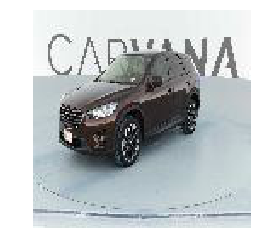
\includegraphics[width = 1.5in]{./new_figs/x_1.png}} &
        \subfloat[Example 2]{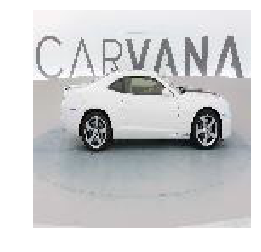
\includegraphics[width = 1.5in]{./new_figs/x_2.png}} &
        \subfloat[Example 3]{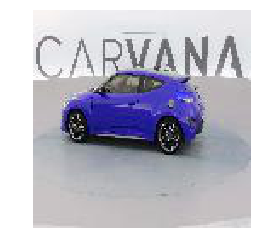
\includegraphics[width = 1.5in]{./new_figs/x_3.png}} &
        \subfloat[Example 4]{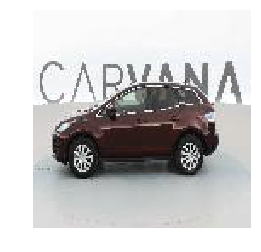
\includegraphics[width = 1.5in]{./new_figs/x_4.png}}
        \end{tabular}
        \caption{Downsampled Image Examples}
        \label{fig:carvana-image-grid}
    \end{figure}
\end{appendixatend}

\begin{appendixatend}
    \subsection{Image Mask Examples}
    \begin{figure}
        \begin{tabular}{cccc}
        \subfloat[Example 1]{
\includegraphics[width = 1.5in]{./new_figs/y_1.png}} &
        \subfloat[Example 2]{
\includegraphics[width = 1.5in]{./new_figs/y_2.png}} &
        \subfloat[Example 3]{
\includegraphics[width = 1.5in]{./new_figs/y_3.png}} &
        \subfloat[Example 4]{
\includegraphics[width = 1.5in]{./new_figs/y_4.png}}
        \end{tabular}
        \caption{Downsampled Mask Examples}
        \label{fig:carvana-mask-grid}
    \end{figure}
\end{appendixatend}

\subsection{Formal Description of Task}

Here is a mathematical description of our task.  Given a dataset $\mathcal{D}$
composed of images, $x \in \mathbb{R}^{d}$, we'd like to learn a function $f :
\mathbb{R}^{d} \mapsto \mathbb{N}$ mapping each input image to
a discrete color label in the natural numbers.  It is key to understand that
this task uses image mask segmentation as an intermediate; more formally,
given a dataset $\mathcal{D}$ composed of images, $x \in \mathbb{R}^{d}$, we'd
like to learn a function $f : \mathbb{R}^{d} \mapsto \{0, 1\}^{d}$, mapping
each pixel to a 0 (for background) or 1 (for foregroud, meaning part of the car)

\subsection{Segmentation Metric}

For this task, we decided to use the F1 metric. The F1 metric is defined as follows:
\begin{equation}
    F1 = \frac{2*precision*recall}{precision + recall}
\end{equation}
where
\begin{equation}
    precision = \frac{TP}{TP + FP}
\end{equation}
and
\begin{equation}
    recall = \frac{TP}{TP + FN}
\end{equation}

\section{Methods}

Our pipeline consists of a few distinct steps.  We begin with aggressive
downsampling, intended to reuce the need for processing power. The result is a
new, smaller dataset ripe for training and inference.

We then pose an intermediary binary classification problem: given a pixel, does
it belong to a car?  To binarize our images, we depend on a type of Deep Neural Network
(DNN) called a U-Net.

With our predicted binary mask, we proceed with the clustering problem: given an image of
a car, what is the color of the car? This is accomplished using DBSCAN preprocessed
with RGB-ratio feature extraction.

\subsection{Downsampling}

After recognizing that 32GB of RAM was not enough to handle the original resolution
of the images, we downsampled from (1918, 1280) to (128, 128). To do so, we used
Pillow's default resize function. An example of such downsampling can be seen in
figure \ref{fig:downsampling}

\begin{appendixatend}
    \subsection{Downsampling Example}
    \begin{figure}
        \begin{tikzpicture}
          \node[inner sep=0pt] (raw) at (0,-13.5)
              {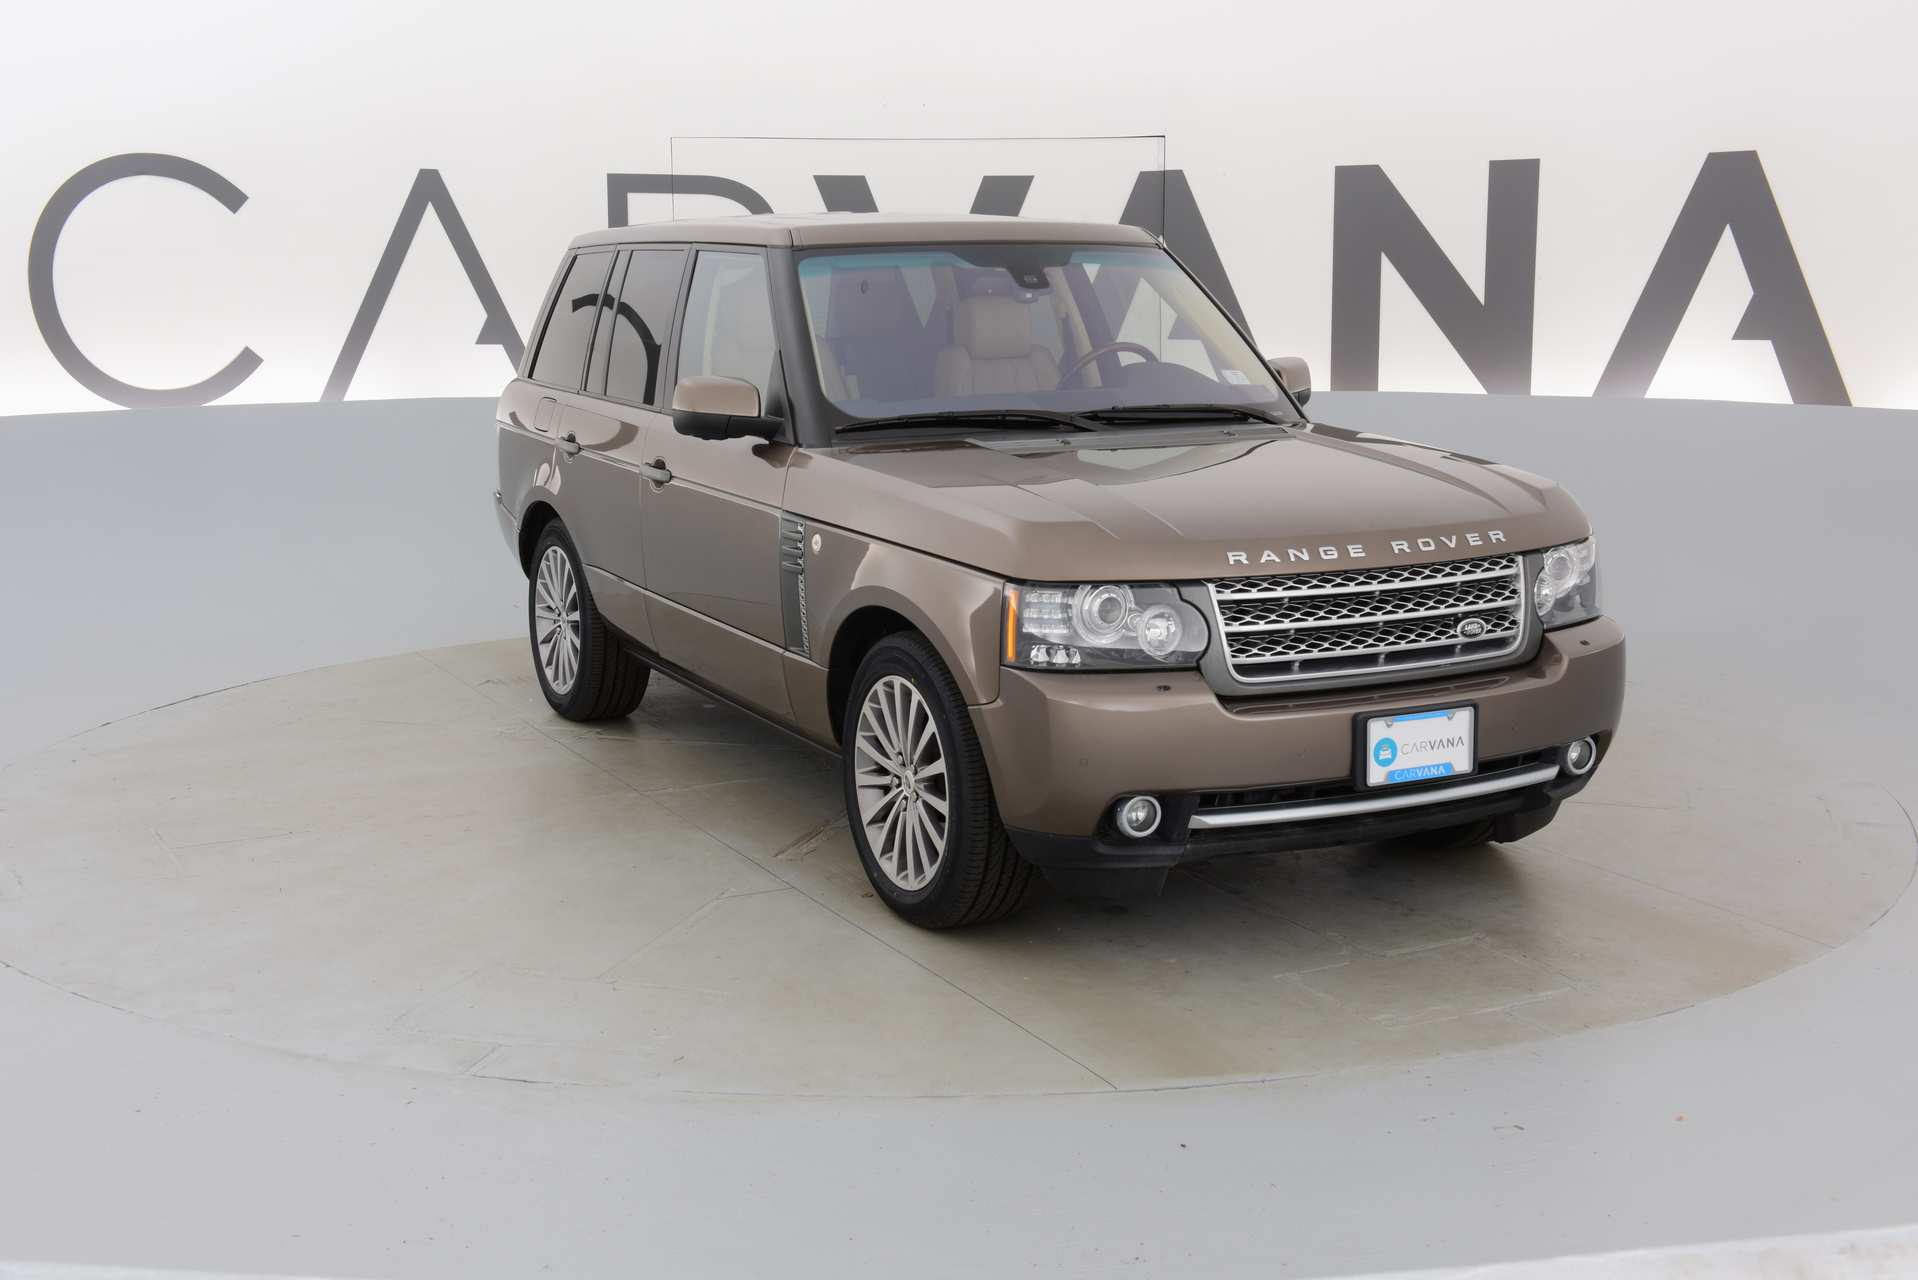
\includegraphics[width=4cm]{./new_figs/raw.jpg}};
          \node[inner sep=0pt] (raw lbl) at (0,-15.5)
              {Original Image};
          \node[inner sep=0pt] (downsample) at (10,-13.5)
              {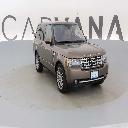
\includegraphics[width=4cm]{./new_figs/downsampled.jpg}};
          \node[inner sep=0pt] (downsample lbl) at (10,-16)
              {Downsampled Image};
          \draw[->,line width=2pt] (raw.east) -- (downsample.west);
        \end{tikzpicture}
        \caption{An example of our image downsampling.}
        \label{fig:downsampling}
    \end{figure}
\end{appendixatend}

\subsection{U-Net as a Learned Binarizer}

Stacking our predictions from our linear models with our 5 features, we complete
our pipeline using a DNN functioning as a learned binarizer called a ``U-Net"
\footnote{\href{https://arxiv.org/pdf/1505.04597.pdf}{The Original U-Net Proposition Paper}}.
The goal of the U-Net is to segment the image. That is, the U-Net learns a function
$f : \mathbb{R} \mapsto \{0, 1\}$ for each pixel such that a class label is assigned
to each pixel. For the purpose of our pipeline, the classes are
\begin{enumerate}
  \item $0$ if we predict a pixel is not part of a car
  \item $1$ if we predict a pixel is part of a car
\end{enumerate}
A plot of the training accuracy and loss per epoch can be found in figure \ref{fig:training_info}.

\begin{appendixatend}
    \subsection{Training Accuracy and Loss During Training}
    \begin{figure}
      \begin{tabular}{cccc}
        \subfloat[UNet Train/Validation Accuracy History]{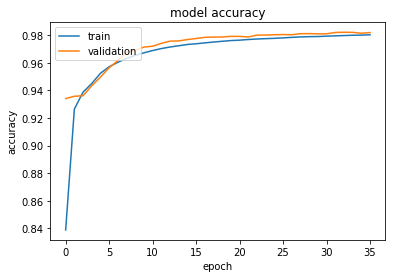
\includegraphics[width = 3in]{./new_figs/train_accuracy_history.png}} &
        \subfloat[UNet Train/Validation Loss History]{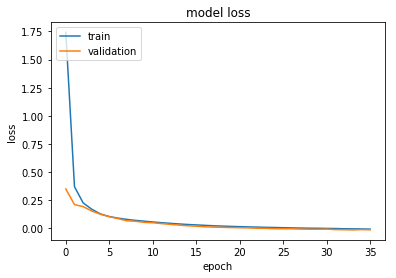
\includegraphics[width = 3in]{./new_figs/train_loss_history.png}}
        \end{tabular}
        \caption{The training loss and accuracy per epoch}
        \label{fig:training_info}
    \end{figure}
\end{appendixatend}

\subsubsection{General U-Net Architecture}
To segment the image, a U-Net ``supplement[s] a usual contracting network by
successive layers, where pooling operators are replaced by upsampling
operators. In order to localize, high resolution features from the contracting
path are combined with the upsampled output" \cite{unet}. Stacking
the high-resolution features with the unsampled output results in symmetry
between the expansive path and the contracting path, resulting in a u-shape as
seen in Figure \ref{fig:U-Net-architecture}. For the image borders, U-Net
extrapolates missing information by mirroring the original image accross the
image borders.

\subsubsection{Our U-Net Architecture}
Our U-Net Architecture is very similar to the original U-Net Architecture. The
only modifications were as follows:
\begin{enumerate}
  \item We added Dropout layers at the end of each 2D convolution block with a
  hyper parameter of .5. We chose .5 because it is the hyperparameter recommended
  by Geoff Hinton. These 9 drop out layers helped reduce overfitting by reducing
  the number of parameters updated after each data example.
  \item We added Batch Normalization at the end of each 2D convolution block. Batch normalization
  improves f1 score and train time by reducing covariant shift and minimizing higher order
  interactions between layers. Covariate shift refers to the change in distribution of inputs,
  specifically the change in inputs between interior layers due to changing output of the previous
  layer. When covariate shift is present it means that intermediate layers continually need
  to adapt to the shifting distribution of input which is the output of the layer before.
  Batch normalization reduces covariate shift by centering the mean around zero and scales
  the variance to one. Centering the mean around zero and scaling the variance to one also
  helps reduce higher order interactions between layers which when present causes learning
  rates at later layers to change drastically. By reducing higher order interaction between
  layers batch normalization allows the use of much higher initial learning rates. In effect
  batch normalization allows for much smoother and quicker gradient descent where the model’s
  later layers will have more stable parameters. This effect means the model as a whole will
  be quicker and more likely to finding local minima which is why we see a decreased train
  time with batch normalization and an increased f1 score.

  \item We used early stopping with a patience of 3 for the training process. This
  was simply to reduce overfitting, but also had a positive secondary effect of
  reducing training time.
\end{enumerate}
Other that this
modification, our architecture is exactly that described in
\href{https://arxiv.org/pdf/1505.04597.pdf}{The Original U-Net Proposition
Paper}.  The Keras code to describe the first iteration of our U-Net
architecture was taken from a
\href{https://www.depends-on-the-definition.com/unet-keras-segmenting-images/}{Kaggle Kernel}.

\subsubsection{Why This Architecture?}
U-Net seemed to be the default segmentation network according to several kaggle users.
Furthermore, after training the U-Net, we found that it sufficiently segmented the foreground
to aid the color clustering, thus we decided to use it. Given more time or computing power, we
would have tried to make the network more shallow or deep. Additionally, we would have tried
VGG-segnet and Keras-FCN.

\subsubsection{Hand Designed Features}

We also attempted to map our data into a computer vision and HSV feature-space
with goals of extracting as much information as possible and creating as much
contrast between foreground and background as possible. Thus, we extracted
as many features as we could think of and fed these features into the U-Net.

Below, we describe the information each feature encodes and the intuition behind
including that information:

\begin{enumerate}
  \item Raw RGB Values:
  We first decided the include the RGB values themselves. Several other
  existing pipelines relied solely on the RGB values and performed quite well,
  meaning the RGB values must encode valuable information, so we included them.
  \item  Bilateral Filter:
  A Bilateral Filter convolves the image with a weighted Gaussian kernal. This
  denoises the image, while still preserving the edges. We included it to
  get rid of background salt and pepper.
  \item 50/99 Image Rescaling:
  Image Rescaling widens the data distribution and increases contrast. We grabbed
  the 50th percentile and rescaled everything below and including that value to
  be 0, and we grabbed the 99th percentile and rescaled everything above that
  value to be 1. We included this to increase contrast between foreground and background,
  and to filter out salt and pepper.
  \item Adaptive Histogram Equalization:
  Adaptive Histogram equalization increases contrast locally. We included this
  so that the regressors could recognize smaller nuclei among salt and papper.
  \item Dilation:
  A dilation performs a uniform kernel convolution accross the image, thus
  setting each pixel to be the average of its neighbors and itself. This increases
  the area of each nucleus. We included this so that the regressors could pick
  out small nuclei.
  \item HSV:
  This stands for hue, saturation, and value. This color space describes colors
  (i.e. hue) in terms of their shades (i.e. saturation) and brightness value.

\end{enumerate}

Ultimately, the model using these features overfit and did not generalize very
well to the test set. 

\begin{appendixatend}
    \subsection{U-Net Architecture}
    \begin{figure}
        \centering
        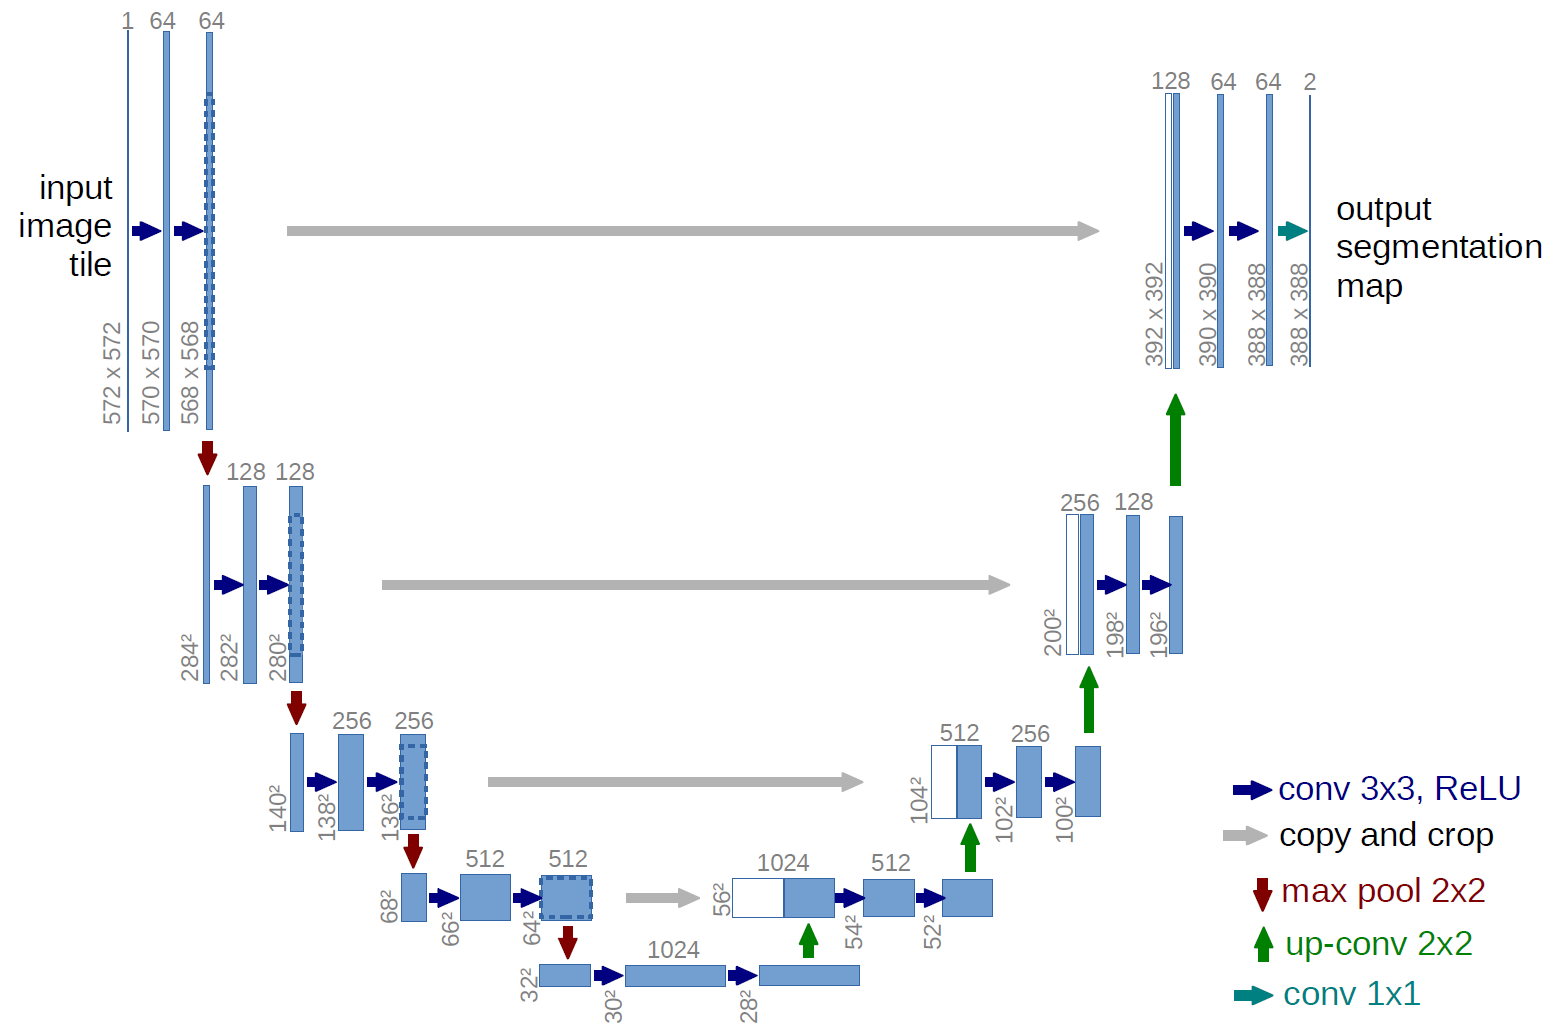
\includegraphics[width=\textwidth]{./figs/unet_architecture.png}
        \caption{The U-Net Architecture, as presented in  \href{https://arxiv.org/pdf/1505.04597.pdf}{The Original U-Net Proposition Paper} }
        \label{fig:U-Net-architecture}
    \end{figure}
\end{appendixatend}

\subsubsection{Shallow Models}
We also attempted to use the following shallow models: Logistic Regression, SVM, and Decision Trees. With each model, we used a validation set to
select the best hyperparameters. However, we found that the best model was an SVM with a train F1 of 0.561 and test F1 of 0.550. Thus, we decided to
use U-Net instead. Intuitively, this is because the majority of the cars in the dataset are black, white or gray, making it very difficult to
distinguish from the grayscale background.

\subsection{Color Clustering}

To cluster the images based off of color, we first fed the image through the U-Net,
finding the foreground mask. An example of such can be found in figure \ref{fig:masking}.
We then applied this mask to the original downsampled image.
We pipelined this step with DBSCAN preprocessed with RGB ratio feature extraction.

\begin{appendixatend}
    \subsection{U-Net Outputs}
    \begin{figure}
    \begin{tabular}{cccc}
    \subfloat[Example 1]{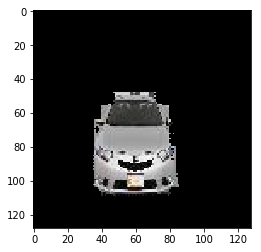
\includegraphics[width = 1.25in]{./new_figs/unet_output1.png}} &
    \subfloat[Example 2]{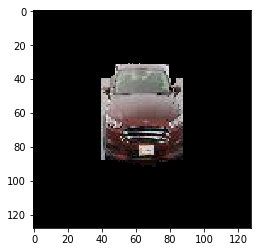
\includegraphics[width = 1.25in]{./new_figs/unet_output2.png}} &
    \subfloat[Example 3]{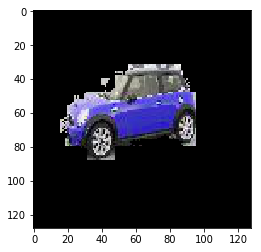
\includegraphics[width = 1.25in]{./new_figs/unet_output3.png}} &
    \subfloat[Example 4]{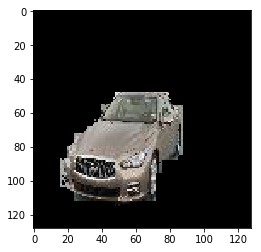
\includegraphics[width = 1.25in]{./new_figs/unet_output4.png}}
    \end{tabular}
    \caption{UNet Output Examples}
    \label{fig:masking}
    \end{figure}
\end{appendixatend}

\subsubsection{RGB Ratio Feature Extraction}
For clustering the cars we used the output of the U-Net to isolate the car itself. Thus, we
could then determine the mean rgb value for each car. In figure \ref{fig:color_plots},
we plot the mean RGB value in for all the cars present in our data set. We then noticed
the data formed a number of linear lines radiating from the origin which would be difficult to seperates
into clusters. And in fact when plotting the clusters produced from raw RGB values, it only clustered the
cars in terms of various shades of gray. We then decided to try to separate the data by taking the ratios
of RGBs. This, we found, created group that could then be cluster. This transformation can also be found
in figure \ref{fig:color_plots}.

\begin{appendixatend}
    \subsection{RGB Ratio Transformation}
    \begin{figure}
      \begin{tikzpicture}
        \node[inner sep=0pt] (raw) at (0,-13.5)
            {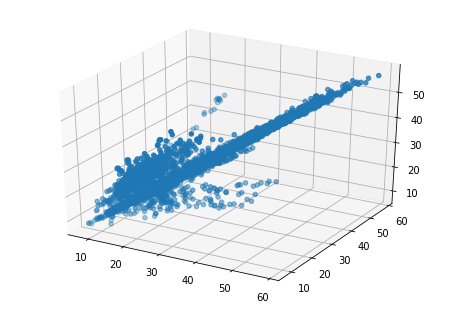
\includegraphics[width=4cm]{./new_figs/colors_3d.png}};
        \node[inner sep=0pt] (raw lbl) at (0,-15.5)
            {RGB Plot};
        \node[inner sep=0pt] (features) at (10,-13.5)
            {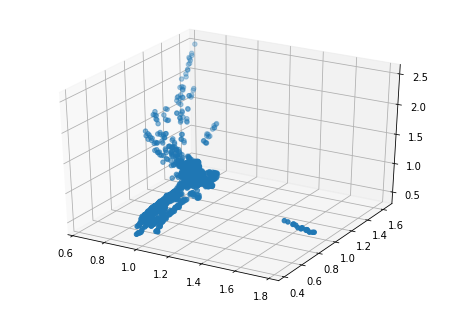
\includegraphics[width=4cm]{./new_figs/color_ratios_3d.png}};
        \node[inner sep=0pt] (features lbl) at (10,-16)
            {RGB Ratio Plot};
        \draw[->,line width=2pt] (raw.east) -- (features.west);
      \end{tikzpicture}
      \caption{A plot of the raw RGB values (left) and the RGB ratios (right)}
    \end{figure}
    \label{fig:color_plots}
\end{appendixatend}

\subsection{ Lessons Learned }

The most important lesson that we learned as a group over the course of this project
is to immediately question a perfect train and test accuracy and the important
 role that visualizing results has in discovering and fixing the error. We
 learned this lesson because of an error we made while splitting our test and
 train data. We split out data such that all pixels not just images were randomly
 assigned to the train or test set. This mistake meant that we were training in
 effect on random noise. We did not realize our error, however, until we decided to
 visualize our findings. By not continually visualizing our outputs we lost a
 considerable amount of time and had to redo work that we thought we were already
 done with. Thankfully the fix was a simple matter of changing the input for our
 test train split function, however, it's still unfortunate that we did not
 realize this error earlier but have in the end learned the importance of
 visualizing your output.


\newpage

\printbibliography

\newpage

\includeappendices

\end{document}
